% -*- mode: latex; -*- mustache tags:  
\documentclass[10pt,twoside,english]{_support/latex/sbabook/sbabook}
\let\wholebook=\relax

\usepackage{import}
\subimport{_support/latex/}{common.tex}

%=================================================================
% Debug packages for page layout and overfull lines
% Remove the showtrims document option before printing
\ifshowtrims
  \usepackage{showframe}
  \usepackage[color=magenta,width=5mm]{_support/latex/overcolored}
\fi


% =================================================================
\title{A PharoThings Tutorial}
\author{Allex Oliveira}
\series{Square Bracket tutorials}

\hypersetup{
  pdftitle = {A PharoThings Tutorial},
  pdfauthor = {Allex Oliveira},
  pdfkeywords = {IoT, Raspberry, PharoThings, Pharo}
}


% =================================================================
\begin{document}

% Title page and colophon on verso
\maketitle
\pagestyle{titlingpage}
\thispagestyle{titlingpage} % \pagestyle does not work on the first one…

\cleartoverso
{\small

  Copyright 2017 by Allex Oliveira.

  The contents of this book are protected under the Creative Commons
  Attribution-ShareAlike 3.0 Unported license.

  You are \textbf{free}:
  \begin{itemize}
  \item to \textbf{Share}: to copy, distribute and transmit the work,
  \item to \textbf{Remix}: to adapt the work,
  \end{itemize}

  Under the following conditions:
  \begin{description}
  \item[Attribution.] You must attribute the work in the manner specified by the
    author or licensor (but not in any way that suggests that they endorse you
    or your use of the work).
  \item[Share Alike.] If you alter, transform, or build upon this work, you may
    distribute the resulting work only under the same, similar or a compatible
    license.
  \end{description}

  For any reuse or distribution, you must make clear to others the
  license terms of this work. The best way to do this is with a link to
  this web page: \\
  \url{http://creativecommons.org/licenses/by-sa/3.0/}

  Any of the above conditions can be waived if you get permission from
  the copyright holder. Nothing in this license impairs or restricts the
  author's moral rights.

  \begin{center}
    
\includegraphics[width=0.2\textwidth]{_support/latex/sbabook/CreativeCommons-BY-SA.pdf}
  \end{center}

  Your fair dealing and other rights are in no way affected by the
  above. This is a human-readable summary of the Legal Code (the full
  license): \\
  \url{http://creativecommons.org/licenses/by-sa/3.0/legalcode}

  \vfill

  % Publication info would go here (publisher, ISBN, cover design…)
  Layout and typography based on the \textcode{sbabook} \LaTeX{} class by Damien
  Pollet.
}


\frontmatter
\pagestyle{plain}

\tableofcontents*
\clearpage\listoffigures

\mainmatter

\chapter{Lesson 8 - I2C Sensors (Temperature, Humidity, Pressure and Acellerometer)}
In the previous lessons, we learned how to control LEDs and to use a button to interact with LEDs. Now let's start using some sensors to interact automatically with the real world, taking the temperature, air pressure and humidity. This kind of sensor use the I2C protocol to communicate.
\section{What we need?}
In this lesson we will use a very simple setup.
\subsection{Components}
\begin{itemize}
\item 1 Raspberry Pi connected to your network (wired or wireless)
\item 1 Breadboard
\item 1 ADXL345 accelerometer sensor
\item 1 BME280 temperature, humidity and pressure sensor
\item 1 MCP9808 temperature sensor
\item Jumper wires
\end{itemize}
\section{Experimental theory}
Before constructing any circuit, you must know the parameters of the components in the circuit, such as their operating voltage, operating circuit, etc.
\subsection{The I2C protocol}
The I2C communication protocol can be easily implemented in many electronic projects, being a very popular and widely used protocol. It is possible to perform communication between one or more master devices and several slave devices. It is an easy-to-implement protocol because it uses only 2 wires to communicate between up to 112 devices using 7-bit addressing and up to 1008 devices using 10-bit addressing.

The Figure \ref{I2CBus} shows how you can connect the devices using the same I2C bus.


\begin{figure}

\begin{center}
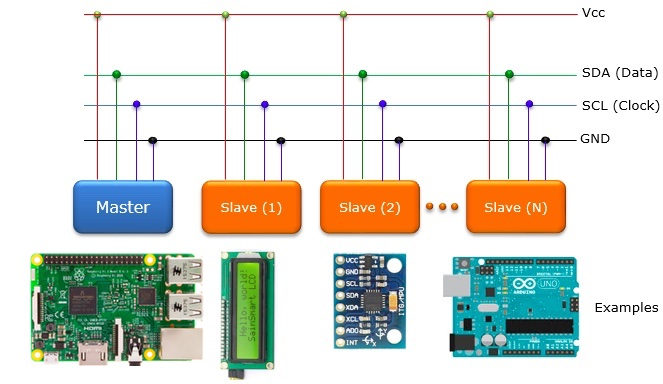
\includegraphics[width=0.8\textwidth]{/Users/allexoliveira/PharoThingsBook/Booklet-APharoThingTutorial/_result/pdf/Chapters/Chap9I2CSensors/figures/pharothings-i2c-bus.jpg}\caption{Devices connected using I2C bus.\label{I2CBus}}\end{center}
\end{figure}

\subsection{How I2C works?}
How can we communicate with multiple devices using only two wires? For this to happen, each device has set an ID or an unique address. Then the master device can choose which device to communicate with.

The two wires are called Serial Clock (or SCL) and Serial Data (or SDA). The SCL wire is the clock signal that synchronizes the data transfer between devices on the I2C bus and is generated by the master device. The other wire is the SDA line that carries the date.
\subsection{Protocol}
The data is transferred in 8-bit sequences, like you can see in Figure \ref{I2CBusPacket}. After a special starting condition occurs, comes the first 8-bit sequence that indicates the address of the slave to which the data is being sent.
For example, for the ADXL345 accelerometer device, the default address is 16r53 (0X53) or 0101 0011 (the last bit actived means the device is on read mode).

After each 8 bit sequence follows a bit called Acknowledge. After the first Acknowledge bit, in most cases another addressing sequence comes, but this time to the internal registers of the slave device. 

The internal registers are locations in the slave's memory containing various information or data. For example, the ADX345 accelerometer has a unique device address (16r53) and addition internal record addresses for the X, Y, and Z axes (16r32, 16r33, 16r34, etc.). Therefore, if we want to read the X-axis data, we first need to send the address of the device and then the internal register address specific to the X-axis.

After the addressing sequences, the data streams are as many as they are sent until the data is completely sent and ends with a special stop condition.


\begin{figure}

\begin{center}
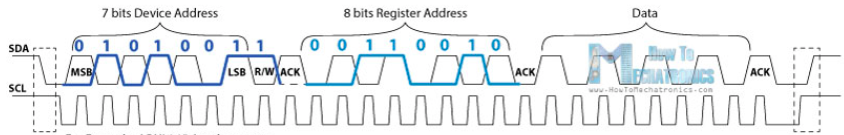
\includegraphics[width=0.8\textwidth]{/Users/allexoliveira/PharoThingsBook/Booklet-APharoThingTutorial/_result/pdf/Chapters/Chap9I2CSensors/figures/pharothings-i2c-bus-data.png}\caption{Bits sequence.\label{I2CBusPacket}}\end{center}
\end{figure}

\section{Experimental procedure}
Now we will build the circuit. This circuit consists of an LED that lights up when power is applied, a resistor to limit current and a power supply (the Rasp).

\begin{itemize}
\item Connect the Ground PIN from Raspberry in the breadboard blue rail (-). Raspeberry Pi models with 40 pins has 8 GPIO ground pins. You can connect with anyone. In this experiment we will use the PIN6 (Ground);
\item Then connect the 3.3V pin in the red rail (+). 
\item Now let's conect the SCL and SDA wires. Connect them like as shown in the Picture ;
\item Now push the sensors in the breadboard;
\item And insert the jumper wires connecting the sensor in the bus, like as shown in the Picture .
\end{itemize}

The Figure \ref{physicalLed} shows how the electric connection is made:
\section{Connecting remotely}
Through your local Pharo image, let’s connect in the Pharo image by running on Raspberry, enable the auto-refresh feature of the inspector, and open the inspector.
Run this code in your local playground:

\begin{displaycode}{plain}
remotePharo := TlpRemoteIDE connectTo: (TCPAddress ip: #[193 51 236 212] port: 40423)
GTInspector enableStepRefresh.
remoteBoard := remotePharo evaluate: [ RpiBoardBRev1 current].
remoteBoard inspect.
\end{displaycode}
\section{Experimental code}
In your inspect window (Inspector on a PotRemoteBoard), let’s create the instances of the firt sensor, .


% lulu requires an empty page at the end. That's why I'm using
% \backmatter here.
\backmatter

% Index would go here

\end{document}
